\dmg{start by describing what you mean by user study... to evaluate linvis we performed a user study...}

\dmg{and you are evaluating the visualizations, NOT the DAG}


We use a controlled mixed-methods users study in order to evaluate the
ability for the DAG to provide users with a conceptual image of how a
commit is integrated into a project, to compare the DAG and \mt models,
and determine which model the users preferred.

In this section, we describe the methods used to for designing and
implementing the user study.
\dmg{no, you describe the study, which includes the methods}

\dmg{Start by giving an overall overview of the study: the study consists of a set of tasks that users are expected to
  perform... do a top down description of what users will do
}

\subsection{Questions and Tasks}
\label{sub:questions}

\dmg{use tasks, not questions. you are asking them to do something that requires an answer, that is different than a question}


\begin{table*}[htpb]
  \centering
  \caption{Conceptual Tasks }
  \label{tab:conceptual_tasks}
  \begin{tabulary}{0.9\textwidth}{LL}
    \toprule
    Task & Description\\
    \midrule
    T1 & Draw a diagram showing how this commit was merged into the master branch, along with any other related commits\\
    T2 & How many individual commits are related to this commit?\\
    T3 & How many merges are involved with merging this commit into the master branch?\\
    \bottomrule
  \end{tabulary}
\end{table*}

\begin{table}[htpb]
  \centering
  \caption{Summarization Tasks}
  \label{tab:summarization_tasks}
  \begin{tabulary}{\linewidth}{LLL}
    \toprule
    Task Set   & Task & Description\\\midrule
    Merge      & T4   & What is the series of merges involved with merging this
    commit?\\
               & T5   & What other commits are merged?\\
    Authorship & T6   & How many authors are involved?\\
               & T7   & Who contributed the most changes?\\
    Files      & T8   & How many files were modified?\\
               & T9   & Which file had the most changes?\\
    Modules    & T10  & Which modules does this merge tree involve?\\
    \bottomrule
  \end{tabulary}
\end{table}

\dmg{avoid editorializing your text: remove purely}

\dmg{watch for tense... we don't begin... the tasks begin... or better, the first tasks...}

The questions and tasks are broken down into four groups. The first two
groups are purely quantitative in nature; the study begins with
conceptual tasks to understand whether the DAG is capable of providing
users with an understanding of how a commit is merged into the master
branch, and other commits that it is merged with. We continue with
summarization tasks, to quantitatively understand if the \mt model makes
a difference in summarization tasks.

The third task set is purely qualitative, \dmg{and are their goal is ... don't imply content in your sentences... be
  precise; this applies to the paragraph before} to gain better understanding
of whether participants preferred working with the \mt model in \tool,
or working with the DAG in Gitk, and what aspects they preferred from
each tool. The final group of questions is simply to gain a better
understanding of the demographic of our participants.


\textbf{Conceptual Tasks}


\dmg{given the choice, not allowed.  I don't understand this section.
  You need to be more top-down in your description. you need to provide
  context on what the users are expected to do, and why. So what are the
  tasks? You never explain.  what is the goal of the tasks? how many?
  what were the tasks? what is expected from each? you need to answer
  these questions, not necessarily in the same order.  also, remember
  this is a comparative study, so I presume the users were asked to do
  both with linvis and without it (choice of gitk/git command line) }

The participants were allowed to use Gitk or the git command line tools
to perform these tasks. These tasks are asked in the specified order,
allowing tabularr to first, create a conceptual understanding of the
commits and merges that will be involved with the rest of the tasks that
follow.tabularmay then use their diagrams to answer T2 and T3. We do not
collect metrics from \tool for the conceptual tasks, opting instead to
determine if the DAG is sufficient for understanding how a commit is
integrated. \tool uses the \mt model show a tree visualization of how
commits are merged, until the commit reaches the master branch.
Table~\ref{tab:conceptual_tasks} shows the conceptual tasks.

\dmg{I don't like the present tense, but that is your option}

We provide the participant with 10 minutes per commit to complete the
first task. The answers to the two other questions in this section are
drawn from the answer in the first task.

\textbf{Summarization Tasks}


\dmg{again, you are going into details first. First the tasks --see
  above-- including their grouping.  then at the end, describe the
  randomization and why it is done (which you did) }

The summarization tasks (Table~\ref{tab:summarization_tasks}) are
grouped into \dmg{how many?} set of tasks according to their theme. The
tasks within a given task set are shuffled, and the task sets are
shuffled, to ensure that similar questions are together, but not in the
same order, and to ensure that the themes are in randomized order
between participants. The order of the commits is shuffled, as well. The
order of the tool is randomized, choosing to start with either \tool or
Gitk, to ensure that we do not place a bias on one tool through the
experiment.

As understanding where the merge begins and ends is vital to answering
the other question, the merge task set will always be the first task set
presented; however, the questions will still be re-ordered within the
task set.

\textbf{User Opinion and Profile}

Finally, we ask the user for their opinions on the tools and for some
information about their level of experience with git.  \dmg{be more
  precise: understanding or preference is too broad. What you want to
  know answers to specific questions regarding how the tools compare and
  which ones they would prefer} The first three questions are intended
to provide us with a better understanding of preference, and insight on
why, the participant had that preference.  The last three questions in
this section are aimed at getting a better understanding of the
demographic of our participants.

\begin{enumerate}
  \item Given these tasks again, which tool would you prefer to use?
  \item Which aspects of each tool did you like and why?
  \item How long have you used git?
  \item If you have used git, for what kind of projects? (personal,
    school courses, professional?)
  \item If you have used git, how many commits, files, and contributors
    were involved with the largest repository you have worked with?
\end{enumerate}


\textbf{Procedure}

\dmg{tell me first why you need to create a script, so I know what you
  do something: we did random assignment of tasks (explain what you did)
  and randomized the order in which the tasks were performed.  Then
  explain why you need a script}

\dmg{it does not randomize the order the tools. It randomizes which tool
  is going to be used on each tasks.  be precise with your language}

\dmg{what you explained how commits relate to tasks and how they get
  assigned? think as if you are explaining this to somebody who has to
  do this: you are the designer, explaining the why and the how }

For each participant, we run a simple python script to generate the
script for the study, eliminating the possibility of bias from us. The
script randomizes the order of the tools, the order of the commits, the
order of the task sets, and the order of the tasks within each task set,
where appropriate.


\subsection{Commit Selection}
\label{sub:commit_selection}

\dmg{see my comments in previous section. it is ok to explain them here,
  but you need to explain what they are briefly in the previous section}

We chose two commits for use in the study. The order that the commits
are presented is randomized between participants, but the order is kept
consistent through the tasks described in the next subsection.

\dmg{this place does not require a description of the database. This
  requires just to say the commits/merge set (dates and numbers are ok)
  only} We use the \tool database, containing commits and merge-tree
information from April 16th 2005 to October 14th, 2014, which
corresponds to being between Linux release 2.6.12-rc3 and Linux
3.17-rc1. \evan{Cite the database even more?} \dmg{again, i have
  problems with your writing: ``we wanted to use in the study commits of
  different size, to determine if the size had an impact in the
  completion of the tasks. We chose commits of three different sizes...}
We chose the commits based on tree sizes. We \dmg{we didn't find: this
  is a fact, not a discovery; what is a majority? 50\%+1? be precise}
\dmg{drop the word inner, and do it in order: 25\% of trees have only
  one commit, 50\%.., 75\%...} found that a majority of the trees
contain at most seven inner commits, while more than 25\% of the trees
contain a single commit. 75\% of the tree contained up to 51 inner
commits and merges, and finally the largest tree contained 7217 nodes.
We chose to work with the trees in \dmg{if you are going to use the
  words quartile, just use them before in your description eg: the
  distribution of the sizes of the trees is x, y merges, whose size
  corresponded to the 25 ,50 quartiles, simple and precisee} the first
and second quartile, as merge trees of sizes between one and seven, not
including the merge into the master branch, make up the majority of the
trees in the database.

\dmg{remove from here, what is here? this is not a road trip :)} From
here, we selected one tree from the trees of a single commit at random.
Selecting a commit from that tree is trivial, as there is only one to
choose.\dmg{remove the obvious, instead concentrate on why the others
  are not trivial}

We selected one tree of size seven at random from all trees of size
seven\dmg{how many where there?}. We placed a restriction the trees, the
selected tree must include at least one internal merge to increase the
complexity of the trees tested. For each randomly selecting a tree, we
chose one of its internal commits at random (using the
\verb|random.choice| function in python 3.6.1).

\dmg{question: so you chose only one commit of each size, and the
  randomization was which tool to use for each question? or did they
  have to do the same task for two commits?}

Using this technique, we selected commit
\emph{a3c1239eb59c0a907f8be5587d42e950f44543f8} from the tree containing
a single node (Figure~\ref{fig:commit_1}), which we will refer to as
\comA, and commit \emph{cdbdd1676a5379f1d5cbd4d476f5e349f445befe}, from
the tree containing seven nodes (Figure~\ref{fig:commit_2}), which we
will refer to as \comB.

\begin{figure}[bpt]
  \centering
\begin{tabular}{ m{1.5cm} m{3cm} }
  
\includegraphics[height=0.5in]{figures/commits/1-commit.pdf} &
  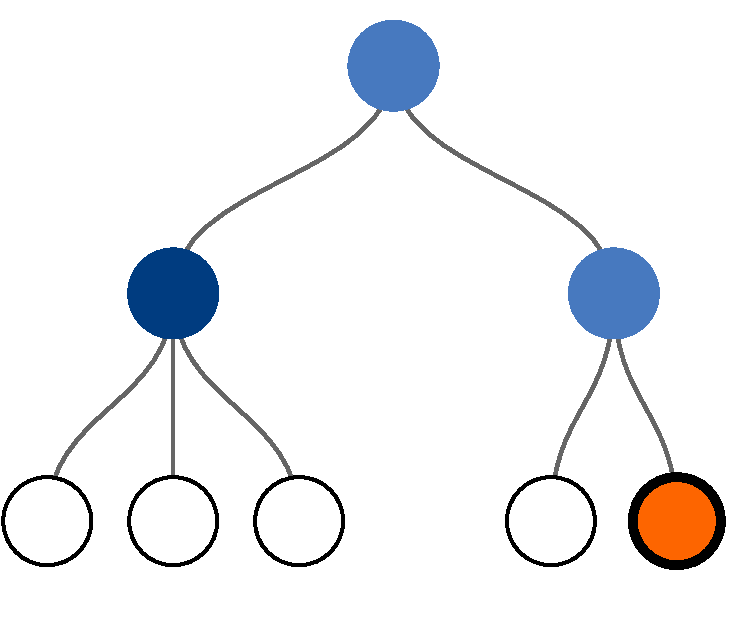
\includegraphics[height=1in]{figures/commits/7-commits.pdf}\\
\end{tabular}
  \caption{The merge trees used in the user study, 
    containing one and seven commits, respectively.}
  \label{fig:commit_1}
\end{figure}


\subsection{Results}
\label{sec:results}

\dmg{this is still methodology.}

We recorded the audio and screen capture video for each participant in
the study for further analysis.
\dmg{you don't need this sentence, it is redundant}
After capturing the information, we
extracted various metrics from the videos.
\dmg{ you don't record, you measure}
From the conceptual tasks, we
recorded the time in seconds, and the answer for the question. We
extracted three metrics for the summarization tasks, the time in
seconds, the correctness, and the accuracy.
\dmg{and then somethings you are over precise :): correctness is simply whether their answer to the task was correct or not}
Correctness is a binary
value, it is true if the response was correct and false if the response
was incorrect.
\dmg{if you are going to use this metric, you need to define precisely. remember, you are giving this to somebody else
  to implement}
The accuracy is measures in distance from the correct
value. An accuracy of zero indicates a correct answer. All tasks in the
summarization tasks include an accuracy metric except T7, which will
only be right or wrong, and therefore cannot meaningfully be measured by
a distance.

\subsection{Conceptual Tasks}
\label{sub:conceptual_tasks}

\dmg{i don't like the expression: we are able to see... too long.. be to the point: Table X shows/depicts/ etc ... they
  are not overviews, they are a summary}
In Table~\ref{tab:conceptual_results}, we are able to see an overview of
the results from the conceptual questions.


\begin{table*}[htpb]
  \centering
  \caption{Results from the conceptual questions\dmg{what are the columns? they need captions}}
  \label{tab:conceptual_results}
  \begin{tabular}{ll|r|lrr|rrr}
    Question                      & Commit & Answer & Median & Mean  & Variance & Median(s) & Mean(s) & Variance(s)\\\hline\hline
    Number of commits in the tree & \comA  & 1      & 4      & 19.11 & 753.11   & 10.0      & 49.92   & 5952.08\\
    Number of merges in the tree  & \comA  & 1      & 5      & 8.27  & 53.62    & 7.5       & 24.67   & 884.42\\\hline
    Number of commits in the tree & \comB  & 5      & 4      & 7.80  & 136.84   & 31.5      & 106.83  & 54123.42\\
    Number of merges in the tree  & \comB  & 3      & 3.5    & 5.40  & 50.27    & 11.0      & 65.6    & 29798.82\\
  \end{tabular}
\end{table*}

Users were able to more closely estimate the number of commits and
merges in the larger tree, but generally took longer than the smaller
tree. The tree with a single node resulted in more variability in the
estimate of number of commits.

It should be noted that these questions were answered after spending
roughly ten minutes attesting to draw a picture that held the answers to
these questions.

\subsection{Summarization Tasks}
\label{sub:summarization_tasks}

In Figure~\ref{fig:summarization_results}, we see all of the
correctness, accuracy, and timing results. The first row of plots are
the correctness results. We see in all cases except for T10, that the
number of instances of a correct result with \tool is roughly the same
as the number of incorrect instances with Gitk. We test each task with
the McNemar Chi-square test~\cite{McNemar1947}.

\begin{figure*}[htpb]
  \centering
  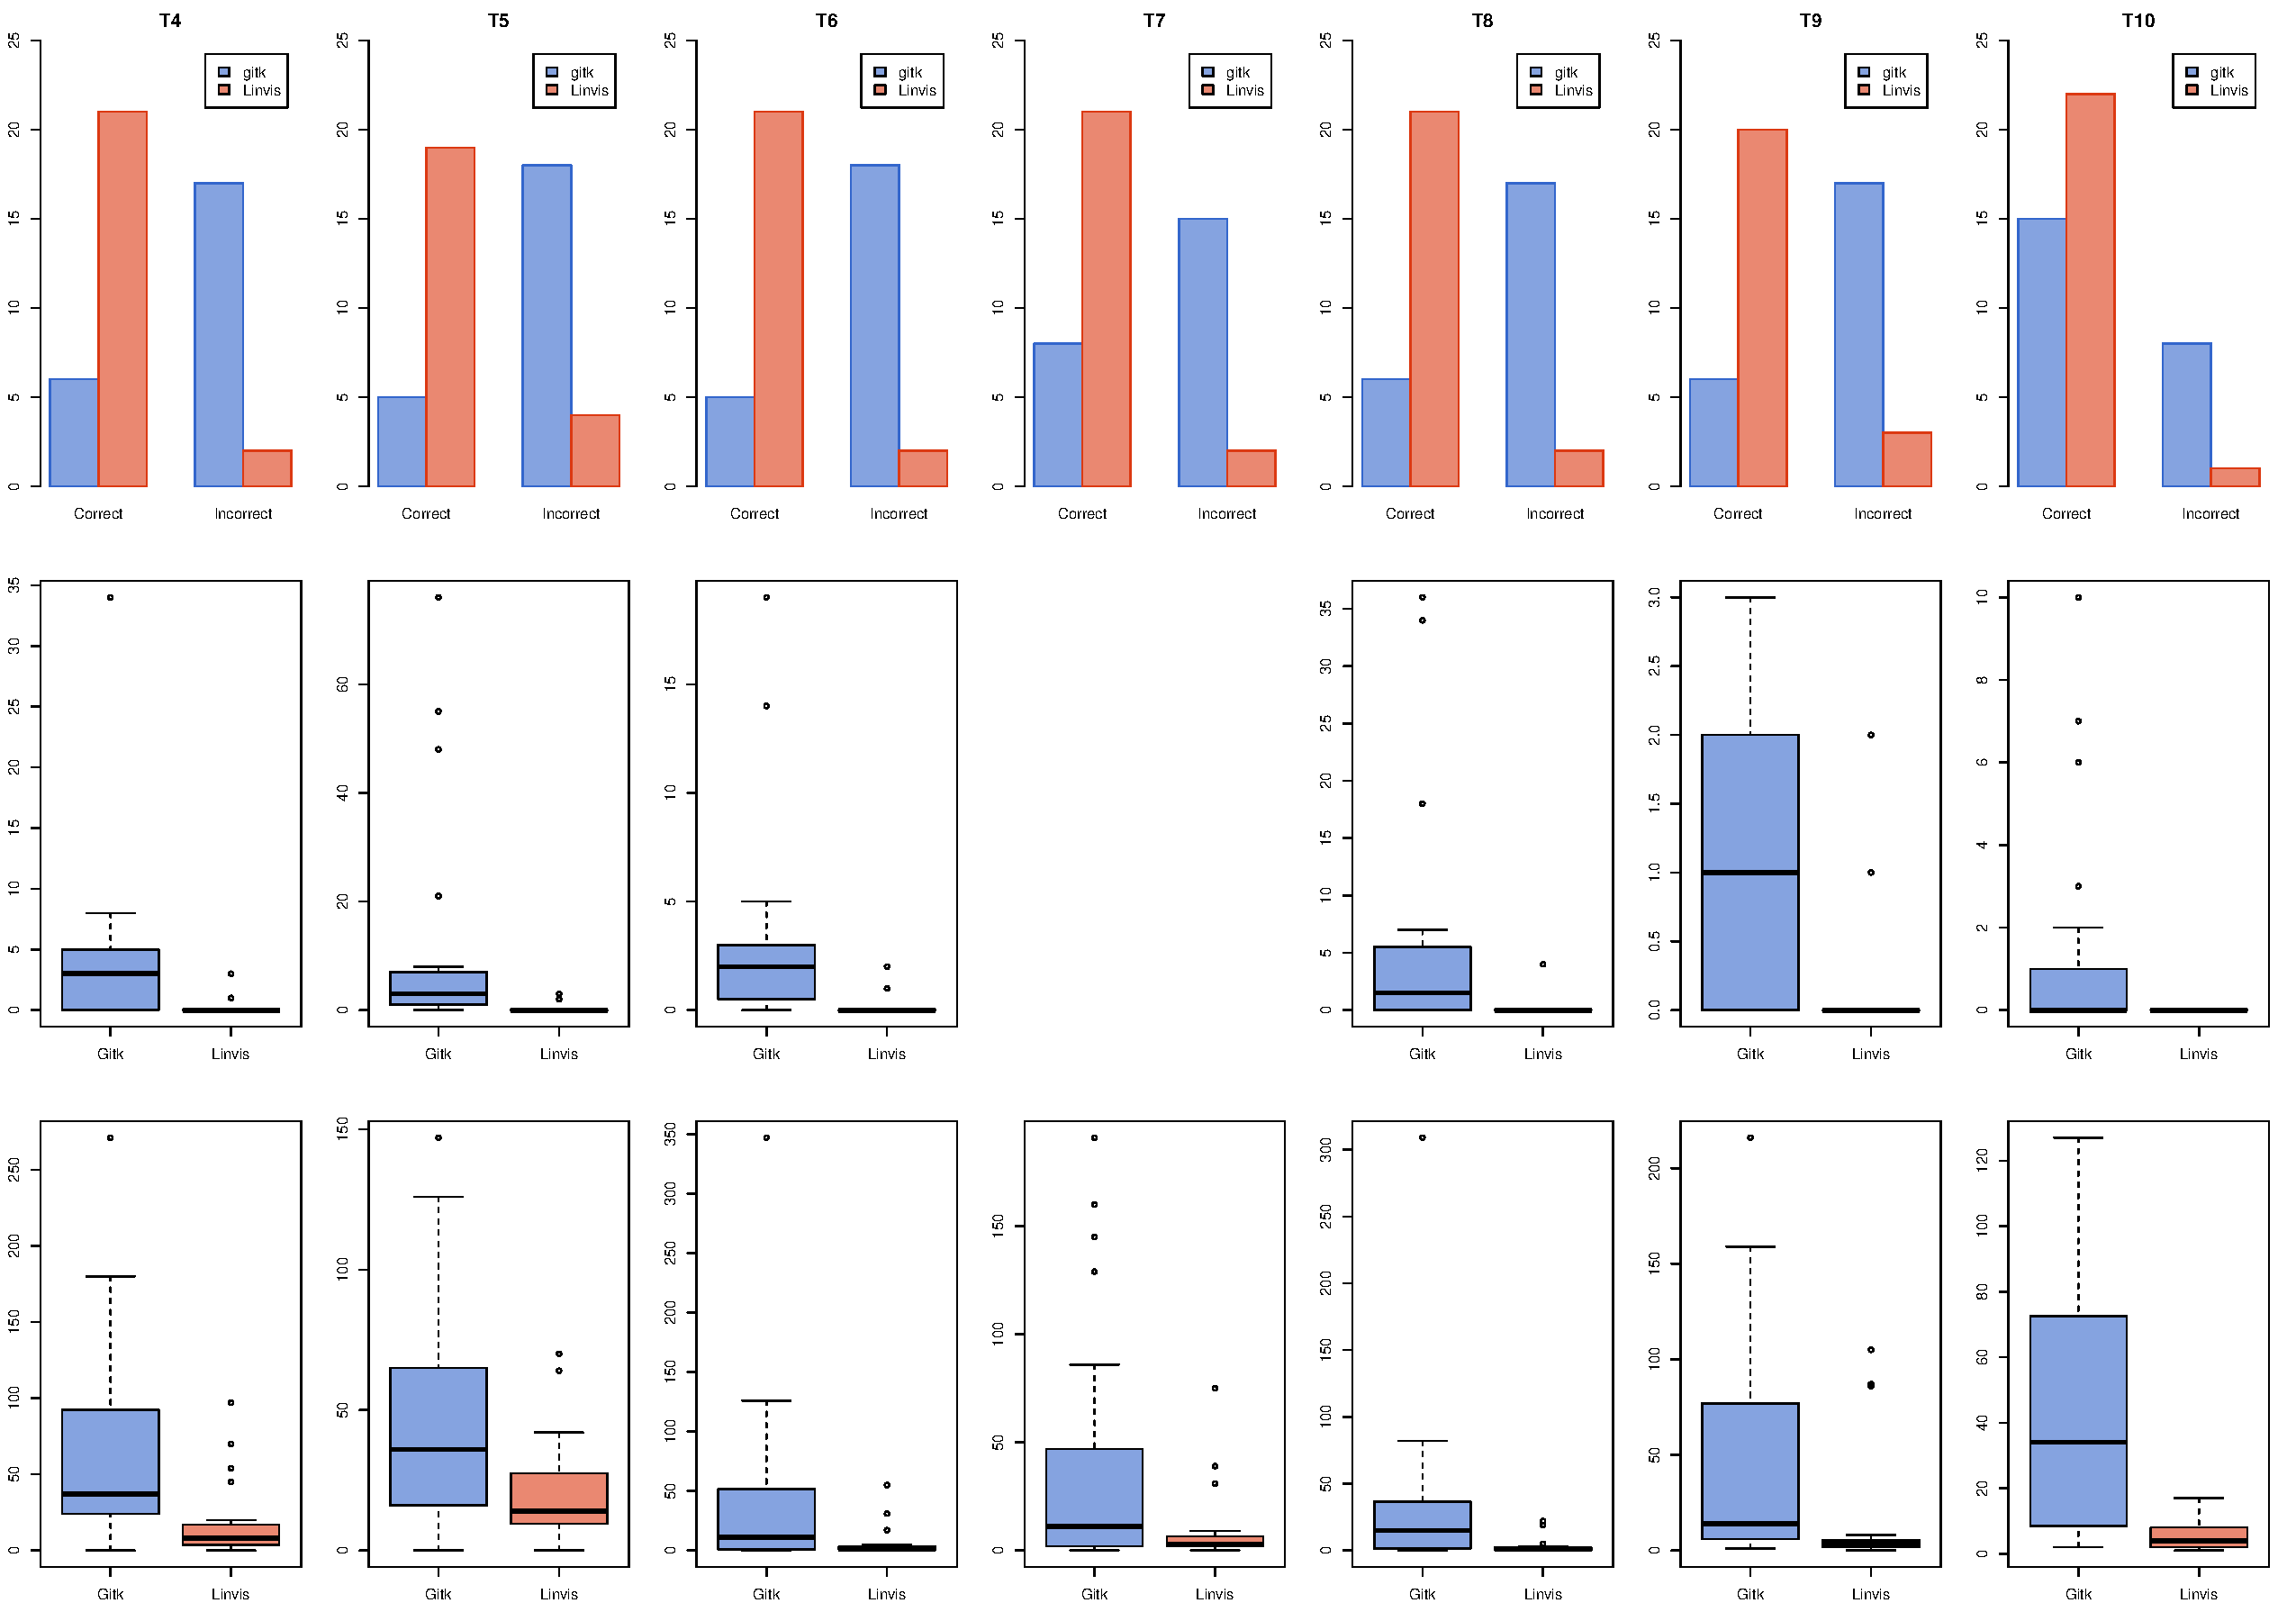
\includegraphics[width=\textwidth]{figures/userstudy/results.pdf}
  \caption{Results from the summarization tasks. The first row plots the
    correctness metric for each task. The second row plots the
    accuracy metric for each task. The third row plots the time metric
    for each task.}
  \label{fig:summarization_results}
\end{figure*}

With the McNemar's tests, we analyze the participants that change from
being correct with one tool to being incorrect with the other. This does
not take into account the number of people who were able to provide the
correct answer for both tools, nor the people who were incorrect for both
tools. The results show whether providing the participants with \tool
over the current standard, gitk, improves the correctness of the
summarization tasks among the participants. We show the results for the
number of people who were, with both tools, correct, incorrect, and
changed in Table~\ref{tab:correctness_table}.

In all cases, except for task T10, we saw statistically significant
results suggesting that we reject the null hypothesis. We tested each
correctness with an $\alpha = 0.005$. The $\chi^2$ test value with one
degree of freedom is $7.879$.

\begin{table*}[htpb]
  \centering
  \caption{Correctness tables showing how many people stayed correct,
    incorrect, and how many people changed between tool}
  \label{tab:correctness_table}
  \begin{tabular}{c|c|c}

    T4 & T5 & T6\\
  \begin{tabular}{cc|rr}
                           &           & \multicolumn{2}{c}{Linvis}\\
                           &           & Correct                      & Incorrect\\\hline
    \multirow{2}{*}{Gitk}  & Correct   & 6                            & 0\\
                           & Incorrect & 15                           & 2\\
  \end{tabular} &

  \begin{tabular}{cc|rr}
                           &           & \multicolumn{2}{c}{Linvis}\\
                           &           & Correct                      & Incorrect\\\hline
    \multirow{2}{*}{Gitk}  & Correct   & 5                            & 0\\
                           & Incorrect & 14                           & 4\\
  \end{tabular}

  &

  \begin{tabular}{cc|rr}
                           &           & \multicolumn{2}{c}{Linvis}\\
                           &           & Correct                      & Incorrect\\\hline
    \multirow{2}{*}{Gitk}  & Correct   & 5                            & 0\\
                           & Incorrect & 16                           & 2\\
  \end{tabular}


  \\\hline
  T7 & T8 & T9\\

  \begin{tabular}{cc|rr}
                           &           & \multicolumn{2}{c}{Linvis}\\
                           &           & Correct                      & Incorrect\\\hline
    \multirow{2}{*}{Gitk}  & Correct   & 8                            & 0\\
                           & Incorrect & 13                           & 2\\
  \end{tabular}  &
  \begin{tabular}{cc|rr}
                           &           & \multicolumn{2}{c}{Linvis}\\
                           &           & Correct                      & Incorrect\\\hline
    \multirow{2}{*}{Gitk}  & Correct   & 6                            & 0\\
                           & Incorrect & 15                           & 2\\
  \end{tabular} &
  \begin{tabular}{cc|rr}
                           &           & \multicolumn{2}{c}{Linvis}\\
                           &           & Correct                      & Incorrect\\\hline
    \multirow{2}{*}{Gitk}  & Correct   & 6                            & 0\\
                           & Incorrect & 14                           & 3\\
  \end{tabular}\\\hline

  & T10 & \\
  & \begin{tabular}{cc|rr}
                            &           & \multicolumn{2}{c}{Linvis}\\
                            &           & Correct                      & Incorrect\\\hline
    \multirow{2}{*}{Gitk}   & Correct   & 14                           & 1\\
                            & Incorrect & 8                            & 0\\
  \end{tabular} & \\

  \end{tabular}
\end{table*}

The correctness test statistics and conclusion for each summarization
task;

The correctness test statistics, conclusions, and a description of the
accuracy and timing results for each summarization task follow:

\begin{itemize}

  \item

    T4; the resulting $\chi^2$ value is $15$. $15 > 7.879$, therefore we
    reject the null hypothesis that \tool does not make a difference in
    the correctness when determining the series of merges that a commit
    takes, with $99.5\%$ confidence.

    There is almost no variation in accuracy between participants using
    \tool, while there is more variance in Gitk. There were two outliers
    among the instances using \tool, which lie within the second and
    third quartiles for the accuracy measure of Gitk. The furthest
    outlier for \tool lies at a distance that is slightly greater than
    the median for Gitk.

    We see similar results in the timing metric; all significant data
    occurs within less time than the second, third, and fourth quartile
    of the Gitk results. Nearly all outlier instances in \tool are
    within the third quartile group of the instances of Gitk with the
    exception of the most extreme, which lies in the fourth quartile
    group.

    The results indicate that \tool is able to assist users with
    determining how a commit is merged more accurately, and more
    quickly.

  \item

    T5; the resulting $\chi^2$ value is $14$. $14 > 7.879$, therefore we
    reject the null hypothesis that \tool does not make a difference in
    the correctness when determining the other related commits, with
    $99.5\%$ confidence.

    There is very little variance in the accuracy of results for \tool
    compared to the accuracy of the results in Gitk. The median distance
    is smaller, indicating that the participants performed more
    accurately using \tool.

    There is less variance in the time taken to come to an answer with
    \tool than with Gitk. Furthermore, we see that a majority of the
    participants were able to complete the task in \tool in much less
    time than 50\% of the participants using Gitk.

    The results indicate that \tool is able to assist users in
    understanding which commits are related to a given commit.

  \item

    T6; the resulting $\chi^2$ value is $16$. $16 > 7.879$, therefore we
    reject the null hypothesis that \tool does not make a difference in
    the correctness when determining the number of authors involved with
    the merge tree, with $99.5\%$ confidence.

    We see the same results from this task as with the previous tasks,
    suggesting that \tool assists users determine the number of authors
    more quickly and more accurately.

  \item

    T7; the resulting $\chi^2$ value is $13$. $13 > 7.879$, therefore we
    reject the null hypothesis that \tool does not make a difference in
    the correctness when determining who contributed the most changes,
    with $99.5\%$ confidence.

    This question does not include an accuracy metric, as there are only
    two possible outcomes. We see the same result in the timing metric
    as we did from the previous questions.

    The results suggest that \tool is able to help users correctly
    identify the person who contributed the most lines of code to a
    merge tree in less time.

  \item

    T8; the resulting $\chi^2$ value is $15$. $15 > 7.879$, therefore we
    reject the null hypothesis that \tool does not make a difference in
    the correctness when determining how many files were contributed,
    with $99.5\%$ confidence.

    The results of this task are the same as in the previous tasks.
    This suggest that \tool is able to assist users determine how many
    files were modified, more quickly and more accurately.

  \item

    T9; the resulting $\chi^2$ value is $14$. $14 > 7.879$, therefore we
    reject the null hypothesis that \tool does not make a difference in
    the correctness when determining which file had the most changes,
    with $99.5\%$ confidence.

    While this question appears to have a similar answer to the correct
    answer for T7, the answer \comA had two files with the same number
    of midifications, thus the participant must correctly identify both
    of these files to be correct. For this reason, we include an
    accuracy metric.

    The results of this task are the same as the previous tasks.
    This suggests that \tool is able to assist users to determine which
    file had the most changes.

  \item

    T10; the resulting $\chi^2$ value is $5.44$. $5.44 < 7.879$,
    therefore we do not reject the null hypothesis, suggesting that
    \tool does not make a difference in determining which modules are
    involved with a merge tree.

    The accuracy and timing results for this task are the same as the
    others, showing that there is less variability in both accuracy and
    the time taken to have an answer between participants using \tool
    than using Gitk. Looking Table~\ref{tab:correctness_table}, we can
    see that, unlike the other questions, a majority of the participants
    were correct using both tools.

\end{itemize}

\subsection{User Opinions}
\label{sub:user_opinions}

Among the 12 pariticipants, there was nearly unanimous agreement that
for conceptual understanding and summarization tasks, \tool was easier
to work with than Gitk. The participants cited the ability to abstract
information about the merge from the clean summarization tables and
simple visualizations. Three participants suggested that someone with a
professional understanding of Gitk and the git commandline may be to
extract the a good conceptual understanding from the DAG, and perform
the summarization tasks from the commandline. One of these three
participants said that they would prefer to have both tools available,
as they are able to complement eachother.

